\clearpage
\subsection{Variable} % (fold)
\label{sub:variable}

A Variable is a \textbf{container} into which you can store a value, which can then be retrieved later. The Variable allows you to store values you want to work with in your program, you store values in the variable so that you can read them back later. The variable's themselves are either a \nameref{sub:global_variable}, \nameref{sub:local_variable}, or \nameref{sub:parameter}.

\begin{figure}[h]
   \centering
   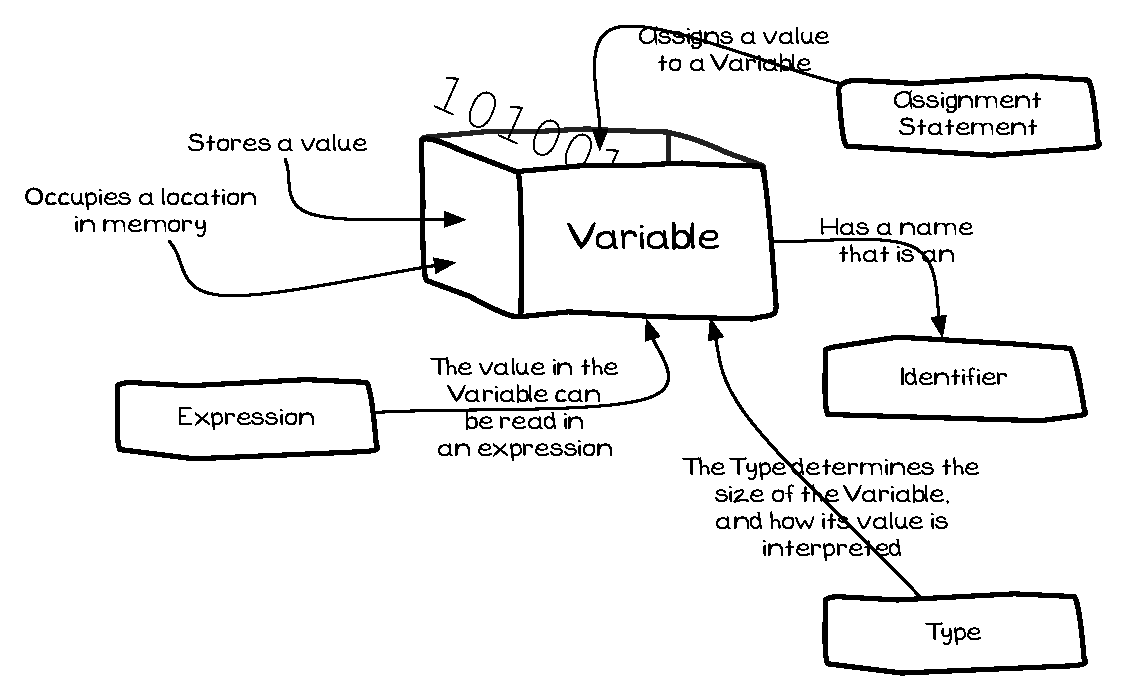
\includegraphics[width=\textwidth]{./topics/storing-using-data/diagrams/Variable} 
   \caption{Variables store a value that can be read and changed}
   \label{fig:storing-using-variable}
\end{figure}

\mynote{
\begin{itemize}
  \item A Variable is an \textbf{artefact}, you can create variables to store values in your programs.
  \item You can think of a Variable like a "box with an item in it". The Variable is the box, its value is the item within it.
  \item Each Variable has a ...
  \begin{itemize}
    \item \textbf{Name} that can be used to refer to it.
    \item \textbf{Value} that it is storing.
    \item \textbf{Type} that determines the size of the Variable and how its value is interpreted.
  \end{itemize}
  \item You use an \nameref{sub:assignment_statement} to store a \emph{value} into the Variable.
  \item You can \textbf{read} the \emph{value} from Variable in Expressions.
  \item The Variable is \textbf{different} to its value:
  \begin{itemize}
    \item The Variable is a container into which a value can be stored.
    \item You can read the \emph{value} from the Variable.
    \item The Variable \textbf{is not} the value, it is a container into which the value is stored.
  \end{itemize}
\end{itemize}
}

% subsection variables (end)